\documentclass[a4paper,12pt]{article}

\usepackage[utf8]{inputenc}
\usepackage[T1]{fontenc}
\usepackage[a4paper,total={150mm,240mm}]{geometry}
\usepackage{amsmath}
\usepackage{amsfonts}
\usepackage{amsthm}
\usepackage{amscd}
\usepackage{grffile}
\usepackage{tikz}
\usetikzlibrary{patterns}
\usepackage{eurosym}
\usepackage{graphicx}
\usepackage{color}
\usepackage{listings}
\lstset{language=C++, basicstyle=\ttfamily,
  keywordstyle=\color{black}\bfseries, tabsize=4, stringstyle=\ttfamily,
  commentstyle=\itshape, extendedchars=true, escapeinside={/*@}{@*/}}
\usepackage{paralist}
\usepackage{curves}
\usepackage{calc}
\usepackage{picinpar}
\usepackage{enumerate}
\usepackage{algpseudocode}
\usepackage{bm}
\usepackage{multibib}
\usepackage{hyperref}
\usepackage{textcase}
\usepackage{nicefrac}

\definecolor{listingbg}{gray}{0.95}

\title{DUNE PDELab Tutorial 02 \\ Cell-Centered Finite Volume Method}
\author{DUNE/PDELab Team}
\date{\today}

\begin{document}

\maketitle
\tableofcontents
\clearpage

\section{Introduction}

This tutorial solves the same partial differential equation (PDE) as tutorial 01, namely
a nonlinear Poisson equation, with the following differences:
\begin{enumerate}[1)]
\item Implements a cell-centered finite volume method with two-point flux
approximation as an example of a non-conforming scheme.
\item Implements \textit{all} possible methods of a local operator.
\end{enumerate}

\subsection*{Depends On} Tutorial 00 and 01.

\section{PDE Problem}

Consider the following nonlinear Poisson equation (the same as in tutorial 01) with
Dirichlet and Neumann boundary conditions:
\begin{subequations} \label{eq:ProblemStrong}
\begin{align}
-\Delta u + q(u) &= f &&\text{in $\Omega$},\\
u &= g &&\text{on $\Gamma_D\subseteq\partial\Omega$},\\
-\nabla u\cdot \nu &= j &&\text{on $\Gamma_N=\partial\Omega\setminus\Gamma_D$}.
\end{align}
\end{subequations}
$\Omega\subset\mathbb{R}^d$ is a domain, $q:\mathbb{R}\to\mathbb{R}$ is a given, possibly
nonlinear function and $f: \Omega\to\mathbb{R}$ is the source term and
$\nu$ denotes the unit outer normal to the domain.

\section{Cell-centered Finite Volume Method}
\label{sec:fv_method}

The application of the cell-centered finite volume method as presented here is
restricted to \textit{axiparallel meshes}. We assume that  the domain $\Omega$ is covered by a mesh
$\mathcal{T}_h = \{T_1, \ldots, T_M\}$ consisting of elements
which are closed sets satisfying
\begin{equation}
\bigcup_{T\in \mathcal{T}_h} T = \overline{\Omega}, \quad
\forall T, T' \in \mathcal{T}_h, T\neq T' : \mathring{T} \cap \mathring{T}' = \emptyset .
\end{equation}
In order to describe the method some further notation is needed.
The nonempty intersections $F = T_F^-\cap T_F^+$
of codimension 1 form the interior skeleton $\mathcal{F}_h^i=\{F_1,\ldots,F_N\}$.
Each intersection is equipped with a unit normal vector $\nu_F$ pointing from $T_F^-$ to $T_F^+$.
The intersections of an element $F=T_F^-\cap\partial\Omega$ with the domain
boundary form the set of boundary intersections $\mathcal{F}_h^{\partial\Omega}=
\{F_1,\ldots,F_L\}$ which can be further partitioned into
Dirichlet boundary intersections $\mathcal{F}_h^{\Gamma_D}$
and Neumann boundary intersections $\mathcal{F}_h^{\Gamma_N}$.
Each boundary intersection is equipped with a unit normal vector
$\nu_F$ which coincides with the unit outer normal to the domain.
Furthermore, $x_T$, $x_F$ denotes the center point of an element or face.
This notation is illustrated graphically in Figure \ref{fig:MeshNotation}.

\begin{figure}
\begin{center}
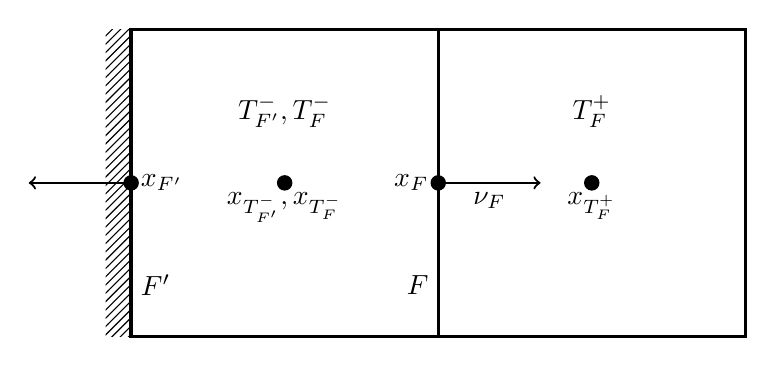
\begin{tikzpicture}[scale=1.3]
\draw[draw=none,pattern=north east lines] (-0.25,0)  rectangle (0,3);
\draw[very thick] (0,0)  rectangle (6,3);
\draw[very thick] (3,0) -- (3,3);
\node at (1.5,2.2) {$T_{F'}^-, T_F^-$};
\node at (4.5,2.2) {$T_F^+$};
\draw[fill=black] (1.5,1.5)  circle (0.07);
\node[below] at (1.5,1.5) {$x_{T_{F'}^-}, x_{T_F^-}$};
\draw[fill=black] (4.5,1.5)  circle (0.07);
\node[below] at (4.5,1.5) {$x_{T_F^+}$};
\draw[thick,->] (3,1.5) -- (4,1.5);
\draw[fill=black] (3,1.5)  circle (0.07);
\node[left] at (3,1.5) {$x_{F}$};
\node[below] at (3.5,1.5) {$\nu_F$};
\node[left] at (3,0.5) {$F$};
\draw[fill=black] (0,1.5)  circle (0.07);
\draw[thick,->] (0,1.5) -- (-1,1.5);
\node[right] at (0,1.5) {$x_{F'}$};
\node[right] at (0,0.5) {$F'$};
\end{tikzpicture}\hspace{0.1\textwidth}
\end{center}
\caption{Illustration of quantities associated with elements and intersections.}
\label{fig:MeshNotation}
\end{figure}

For the cell-centered finite volume method the discrete function space involved
is the space of piecewise constant functions on the mesh:
\begin{equation*}
W_h = \{w\in L^2(\Omega) \,:\,  \text{$w|_T=$ const for all $T\in\mathcal{T}_h$}\} .
\end{equation*}

In order to derive the residual form we proceed as follows: multiply
equation \eqref{eq:ProblemStrong} with a test function $v\in W_h$, i.e. \textit{from
the discrete space}, and use integration by parts:
\begin{align*}
\int_{\Omega} f v \,dx &= \int_{\Omega} [-\Delta u + q(u)] v\,dx\\
&= \sum_{T\in\mathcal{T}_h} v \int_T -\Delta u + q(u) \,dx &&\text{($v$ const on $T$)}\\
&= \sum_{T\in\mathcal{T}_h} \left[\int_T q(u) v \,dx - \int_{\partial T} \nabla u \cdot \nu v \,ds
\right] &&\text{(Gauss' thm.)} \\
&= \sum_{T\in\mathcal{T}_h} \int_T q(u) v \,dx
-\sum_{F\in\mathcal{F}_h^i} \int_F \nabla u \cdot \nu_F \bigl[v(x_{T_F^-}) - v(x_{T_F^+})\bigr] \,ds \\
& \hspace{10mm}-\sum_{F\in\mathcal{F}_h^{\partial\Omega}} \int_F \nabla u \cdot \nu_F \,ds .
&&\text{(rearrange)}
\end{align*}
At this point, the normal derivative $\partial_{\nu_F} u = \nabla u\cdot \nu_F$
is approximated by a difference quotient
\begin{equation*}
\nabla u\cdot \nu_F = \frac{u_h(x_{T_F^+})-u_h(x_{T_F^-})}{\|x_{T_F^+} - x_{T_F^-}\|}
 + \text{ error}
\end{equation*}
and all integrals are approximated by the midpoint rule
\begin{equation*}
\int_T f \,dx = f(x_T)|T| + \text{ error}
\end{equation*}
where $|T|$ is the measure of $T$.

Put together the cell-centered finite volume method can be stated
in its abstract form suitable for implementation in PDELab:
\begin{equation}
\boxed{ \text{Find $u_h\in W_h$ s.t.:} \quad r_h^{\text{CCFV}}(u_h,v) = 0 \quad \forall v \in W_h }
\end{equation}
where the residual form is
\begin{equation}
\label{eq:res_form_final}
\begin{split}
r_h^{\text{CCFV}}(u_h,v)
& = \sum_{T\in\mathcal{T}_h} q(u_h(x_T)) v(x_T) |T|
- \sum_{T\in\mathcal{T}_h} f(x_T) v(x_T) |T|\\
&\ - \sum_{F\in\mathcal{F}_h^i}
\frac{u_h(x_{T_F^+})-u_h(x_{T_F^-})}{\|x_{T_F^+} - x_{T_F^-}\|}
\bigl[v(x_{T_F^-}) - v(x_{T_F^+})\bigr] |F|\\
&\ + \sum_{F\in\mathcal{F}_h^{\partial\Omega}\cap\Gamma_D}
\frac{u_h(x_{T_F^-})}{\|x_{F} - x_{T_F^-}\|} v(x_{T_F^-}) |F| \\
&\ - \sum_{F\in\mathcal{F}_h^{\partial\Omega}\cap\Gamma_D}
\frac{g(x_{F})}{\|x_{F} - x_{T_F^-}\|} v(x_{T_F^-}) |F|
+ \sum_{F\in\mathcal{F}_h^{\partial\Omega}\cap\Gamma_N} j(x_{F}) v(x_{T_F^-}) |F| .
\end{split}
\end{equation}
In this case \textit{five} different types of integrals are involved in the
residual form:
\begin{enumerate}
\item Volume integral depending on trial and test function.
\item Volume integral depending on test function only.
\item Interior intersection integral depending on trial and test function.
\item Boundary intersection integral depending on trial and test function.
\item Boundary intersection integral depending on test function only.
\end{enumerate}
Also note that no constraints on the function space are necessary in this case.
Dirichlet as well as Neumann boundary conditions are built weakly into the
residual form!

Finally, many types of discontinuous Galerkin finite element methods (DGFEM)
lead to the same five types of integrals and can be applied on general unstructured
conforming as well as nonconforming meshes.

\subsection*{General Residual Form}

The residual form of the cell-centered finite volume method suggests that
all residual forms could be composed of five different types of terms
in the following way:
\begin{equation}
\begin{split}
r(u,v) &=
\sum_{T\in\mathcal{T}_h} \alpha_T^V(R_T u, R_T v)
+ \sum_{T\in\mathcal{T}_h} \lambda_T^V(R_T v) \\
&\qquad+ \sum_{F\in\mathcal{F}_h^i} \alpha_F^S(R_{T_F^-} u,R_{T_F^+} u, R_{T_F^-} v, R_{T_F^+} v)\\
&\qquad+ \sum_{F\in\mathcal{F}_h^{\partial\Omega}} \alpha_F^B(R_{T_F^-} u, R_{T_F^-} v)
+ \sum_{F\in\mathcal{F}_h^{\partial\Omega}} \lambda_F^B(R_{T_F^-} v) .
\end{split}\label{eq:GeneralResidualForm}
\end{equation}
Here, we define the restriction
of a function $u\in U$ to an element by
\begin{equation*}
(R_T u)(x) = u(x) \quad \forall x\in\mathring{T} .
\end{equation*}
Note that the restriction of a function to element $T$ is only defined in
the interior of $T$. On interior intersections $F$, functions may be two-valued
and limits from within the elements $T_F^-, T_F^+$ need to be defined
(when $U$ is the space of element-wise constants that is trivial).

The five terms comprise volume integrals (superscript $V$), interior skeleton integrals
(superscript $S$) and boundary integrals (superscript $B$). Furthermore, the
$\alpha$-terms depend on trial and test functions whereas the $\lambda$-terms only
depend on the test function and involve the data of the PDE.

Each of the five terms $\alpha_T^V$, $\alpha_F^S$, $\alpha_F^B$,
$\lambda_T^V$, $\lambda_F^B$ corresponds to one method on the
local operator.
In addition to the evaluation of residuals also Jacobians and
matrix-free application of Jacobians are needed. This gives rise
to in total $5+3+3=11$ possible methods on a local operator given in the following table:
\begin{center}
\footnotesize
\begin{tabular}{l|l|l|l}
    & volume & skeleton & boundary \\
\hline
residual    & \lstinline!alpha_volume! & \lstinline!alpha_skeleton! & \lstinline!alpha_boundary! \\
                & \lstinline!lambda_volume! & & \lstinline!lambda_boundary! \\
\hline
Jacobian  & \lstinline!jacobian_volume! & \lstinline!jacobian_skeleton! & \lstinline!jacobian_boundary! \\
\hline
Jac.  app.  & \lstinline!jacobian_apply_volume! & \lstinline!jacobian_apply_skeleton! &
\lstinline!jacobian_apply_boundary!
\end{tabular}
\end{center}

\section{Realization in PDELab}

The structure of the code is already known from the previous tutorials.
It consists of the following files:
\begin{enumerate}[1)]
\item The ini-file
\lstinline{tutorial02.ini} holds parameters read by various parts of the code
which control the execution.
\item The main file \lstinline{tutorial02.cc} includes the necessary C++,
DUNE and PDELab header files
and contains the \lstinline{main} function where the execution starts.
The purpose of the \lstinline{main} function is
to instantiate DUNE grid objects and call the \lstinline{driver} function.
\item File \lstinline{driver.hh} instantiates the necessary PDELab classes
for solving a nonlinear stationary problem with the cell-centered finite
volume method and solves the problem.
\item File \lstinline{nonlinearpoissonfv.hh} contains the class
\lstinline{NonlinearPoissonFV} realizing a PDELab local operator implementing
the cell-centered finite volume method on axi-parallel meshes.
\item File \lstinline{problem.hh} contains a parameter class which
encapsulates the user-definable part of the PDE problem as introduced in
tutorial 01.
\end{enumerate}

\subsection{Ini-File}

The ini-file uses the same sections as in tutorial 01 with the following exceptions:
\begin{itemize}
\item Only the structured grid in its \lstinline{YaspGrid} implementation can be used
in dimension 2 and 3. \lstinline{OneDGrid} is used in dimension 1.
\item No degree can be chosen.
\end{itemize}

\subsection{Function \lstinline{main}}

The function \lstinline{main} is very similar to the one in tutorials 00 and 01
and need not be repeated here.

\subsection{Function \lstinline{driver}}

Also the function \lstinline{driver} is very similar in structure to the
one in tutorial 00 and 01. Here we just point out the differences.
The cell-centered finite volume method is based on the space of piecewise
constant functions on the mesh $W_h$. The following code segment
constructs this function space using the class \lstinline{P0LocalFiniteElementMap}:
\lstinputlisting[linerange={20-27},
basicstyle=\ttfamily\small,
frame=single,
backgroundcolor=\color{listingbg}]{../src/driver.hh}
The constraints class \lstinline{NoConstraints} is used to express that
there are no constraints on the function space.

Now no constraints container type is exported by the grid function space.
Instead the class \lstinline{EmptyTransformation} is used in the grid operator:
\lstinputlisting[linerange={44-55},
basicstyle=\ttfamily\small,
frame=single,
backgroundcolor=\color{listingbg}]{../src/driver.hh}

Cell-wise data is passed to the \lstinline{VTKWriter}
using its method \lstinline{addCellData}:
\lstinputlisting[linerange={66-72},
basicstyle=\ttfamily\small,
frame=single,
backgroundcolor=\color{listingbg}]{../src/driver.hh}
These are the only changes to the driver!

\subsection{The \lstinline{Problem} Class}

The class \lstinline{NonlinearPoissonFV} explained below uses
the same problem class as the class \lstinline{NonlinearPoissonFEM}. This means
that the same problem can be easily solved using the two different methods.

\subsection{Local Operator \lstinline{NonlinearPoissonFV}}

The class \lstinline{NonlinearPoissonFV} implements the
element-wise computations of the cell-centered finite volume
method. In particular, it provides a full implementation
of all possible methods on a local operator including
analytic Jacobians. The class has the problem class as a template parameter:
\lstinputlisting[linerange={23-27},
basicstyle=\ttfamily\small,
frame=single,
backgroundcolor=\color{listingbg}]{../src/nonlinearpoissonfv.hh}
The base class \lstinline{FullSkeletonPattern} provides the local operator
with a method coupling all degrees of freedom of two elements sharing an intersection.
In combination with \lstinline{FullVolumePattern} this provides the sparsity pattern
of the matrix.

The only private data member is a reference to an object
to the parameter class:
\lstinputlisting[linerange={29-29},
basicstyle=\ttfamily\small,
frame=single,
backgroundcolor=\color{listingbg}]{../src/nonlinearpoissonfv.hh}

The public section begins with a definition of flags controlling
assembly of the sparsity pattern
\lstinputlisting[linerange={32-34},
basicstyle=\ttfamily\small,
frame=single,
backgroundcolor=\color{listingbg}]{../src/nonlinearpoissonfv.hh}
as well as element contributions:
\lstinputlisting[linerange={36-41},
basicstyle=\ttfamily\small,
frame=single,
backgroundcolor=\color{listingbg}]{../src/nonlinearpoissonfv.hh}
These five flags specify that all five contributions will be provided.

The constructor just gets a reference of the parameter object:
\lstinputlisting[linerange={44-44},
basicstyle=\ttfamily\small,
frame=single,
backgroundcolor=\color{listingbg}]{../src/nonlinearpoissonfv.hh}

\subsubsection*{Method \lstinline{lambda_volume}}

This method was already present in the finite element method
and corresponds
to sum number two on the right hand side of equation \eqref{eq:res_form_final}.
The element contributions for the cell-centered finite volume method are
particularly simple to implement. Here is the right hand side contribution:
\lstinputlisting[linerange={49-61},
basicstyle=\ttfamily\small,
frame=single,
backgroundcolor=\color{listingbg}]{../src/nonlinearpoissonfv.hh}
The variable \lstinline{cellcenterlocal} is filled with the
center of the reference element. Then the function $f$ is evaluated
and the integral is approximated with the midpoint rule.
To that end \lstinline{cellgeo.volume()} provides the measure
of the element.

Note that throughout the whole class we assume that the basis
functions of the space $W_h$ are one on one element and zero on
all others, i.e.
\begin{equation}
\phi_i(x) = \left\{ \begin{array}{ll} 1 & x\in T_i \\ 0 & \text{else} \end{array}
\right . .
\end{equation}
This means that basis functions will never be evaluated!

\subsubsection*{Method \lstinline{lambda_boundary}}

This method was also already present in the finite element method
and corresponds
to sums five \textit{and} six on the right hand side of equation \eqref{eq:res_form_final}.
It assembles contributions from Dirichlet and Neumann
boundary conditions and has the interface
\lstinputlisting[linerange={64-66},
basicstyle=\ttfamily\small,
frame=single,
backgroundcolor=\color{listingbg}]{../src/nonlinearpoissonfv.hh}

First  the center of the reference element of the intersection
is extracted and the boundary condition type is evaluated:
\lstinputlisting[linerange={68-75},
basicstyle=\ttfamily\small,
frame=single,
backgroundcolor=\color{listingbg}]{../src/nonlinearpoissonfv.hh}

Now comes the part for the Dirichlet boundary conditions where we
need to compute the distance from the face center to the element center,
the value of the Dirichlet boundary condition and the measure of the face:
\lstinputlisting[linerange={77-100},
basicstyle=\ttfamily\small,
frame=single,
backgroundcolor=\color{listingbg}]{../src/nonlinearpoissonfv.hh}
The Neumann part is much simpler:
\lstinputlisting[linerange={101-106},
basicstyle=\ttfamily\small,
frame=single,
backgroundcolor=\color{listingbg}]{../src/nonlinearpoissonfv.hh}

\subsubsection*{Method \lstinline{alpha_volume}}

Now \lstinline{alpha_volume} has also been present before and corresponds
to the first sum on the right hand side of equation \eqref{eq:res_form_final}.
Here it just contains the evaluation of the reaction term
with the midpoint rule:
\lstinputlisting[linerange={110-123},
basicstyle=\ttfamily\small,
frame=single,
backgroundcolor=\color{listingbg}]{../src/nonlinearpoissonfv.hh}

\subsubsection*{Method \lstinline{jacobian_volume}}

Now we come to the first method that has not been implemented in
previous examples. The method \lstinline{jacobian_volume}
will assemble the entries of the Jacobian coupling all degrees of
the given element. As there is only one degree of freedom per element there
is only one matrix entry to assemble. The matrix entries are returned
in the container which is the last argument of the method:
\lstinputlisting[linerange={126-129},
basicstyle=\ttfamily\small,
frame=single,
backgroundcolor=\color{listingbg}]{../src/nonlinearpoissonfv.hh}

First the derivative of the nonlinearity is evaluated
\lstinputlisting[linerange={132-133},
basicstyle=\ttfamily\small,
frame=single,
backgroundcolor=\color{listingbg}]{../src/nonlinearpoissonfv.hh}
and the matrix entry is written into the container
\lstinputlisting[linerange={136-136},
basicstyle=\ttfamily\small,
frame=single,
backgroundcolor=\color{listingbg}]{../src/nonlinearpoissonfv.hh}
\lstinline{mat.accumulate} has five arguments:
the \textit{matrix row} given by local test space and number of the
test function, the \textit{matrix column} given by local trial space and
number of the trial function and, as last argument, the contribution to
the matrix entry which is added to the global Jacobian matrix.

\subsubsection*{Method \lstinline{jacobian_apply_volume}}

This method is very similar to the previous method except that
it multiplies the local Jacobian contribution immediately with a vector
and accumulates the result.

The method has the following interface:
\lstinputlisting[linerange={140-144},
basicstyle=\ttfamily\small,
frame=single,
backgroundcolor=\color{listingbg}]{../src/nonlinearpoissonfv.hh}
\lstinline{x} are the coefficients of the linearization point and
\lstinline{z} are the entries of the vector to be multiplied with the
Jacobian. The result is accumulated to the container \lstinline{r}.

Here is the implementation:
\lstinputlisting[linerange={146-151},
basicstyle=\ttfamily\small,
frame=single,
backgroundcolor=\color{listingbg}]{../src/nonlinearpoissonfv.hh}
Comparison with \lstinline{jacobian_volume} shows that
the Jacobian entry is multiplied with the entry of \lstinline{z}.

\subsubsection*{Method \lstinline{alpha_skeleton}}

This is the major new method needed to implement the flux terms
in finite volume and discontinuous Galerkin methods. It
has the following interface:
\lstinputlisting[linerange={155-160},
basicstyle=\ttfamily\small,
frame=single,
backgroundcolor=\color{listingbg}]{../src/nonlinearpoissonfv.hh}
The arguments comprise an intersection, local trial function
and local test space for both elements adjacent to the intersection
and containers for the local residual contributions in both elements.
The subscripts \lstinline{_i} and \lstinline{_o} correspond to
``inside'' and ``outside''. W.r.t. our notation above in section \ref{sec:fv_method}
``inside'' corresponds to ``-'' and ``outside'' corresponds to ``+''.

Note that \lstinline{alpha_skeleton} needs to assemble
residual contributions for all test functions involved with \textit{both}
elements next to the intersection and corresponds
to sum number three on the right hand side of equation \eqref{eq:res_form_final}.

It starts by extracting the elements adjacent to the intersection
\lstinputlisting[linerange={163-164},
basicstyle=\ttfamily\small,
frame=single,
backgroundcolor=\color{listingbg}]{../src/nonlinearpoissonfv.hh}
and then extracts their geometries
\lstinputlisting[linerange={167-168},
basicstyle=\ttfamily\small,
frame=single,
backgroundcolor=\color{listingbg}]{../src/nonlinearpoissonfv.hh}
and the centers
\lstinputlisting[linerange={171-172},
basicstyle=\ttfamily\small,
frame=single,
backgroundcolor=\color{listingbg}]{../src/nonlinearpoissonfv.hh}
Now the distance of the centers can be computed
\lstinputlisting[linerange={175-176},
basicstyle=\ttfamily\small,
frame=single,
backgroundcolor=\color{listingbg}]{../src/nonlinearpoissonfv.hh}
and the measure of the face is extracted
\lstinputlisting[linerange={179-180},
basicstyle=\ttfamily\small,
frame=single,
backgroundcolor=\color{listingbg}]{../src/nonlinearpoissonfv.hh}
which puts us in the position to accumulate the residual contributions
\lstinputlisting[linerange={183-185},
basicstyle=\ttfamily\small,
frame=single,
backgroundcolor=\color{listingbg}]{../src/nonlinearpoissonfv.hh}
In fact, the contribution to the inside element, i.e. to \lstinline{r_i} is the flux from the
inside to the outside element. The contribution to the outside
element residual is exactly the negative value, i.e. we have local conservation.

\subsubsection*{Method \lstinline{jacobian_skeleton}}

In the computation of the Jacobian w.r.t. skeleton terms
we can exploit the fact that the discrete residual form is
actually linear in these terms as the nonlinearity is restricted to the
volume term only.

An interior face contributes to four matrix parts of the global matrix as there
are test functions on the inside and outside elements (corresponding to rows in the
matrix) as well as trial functions on the inside and outside element (corresponding to
columns of the matrix). In the case of the cell-centered finite volume method for
the nonlinear Poisson equations there is only one degree of freedom and test function per
element, so there are four matrix entries which the face contributes. In case of higher
order discontinuous Galerkin schemes and/or systems of PDEs there are four blocks
of the matrix where the face contributes to. The following figure illustrates
the matrix structure and the corresponding submatrices. For ease of drawing it is
assumed that all trial and test functions of one element are numbered consecutively
but this need not be the case!
\begin{figure}[h]
\begin{center}
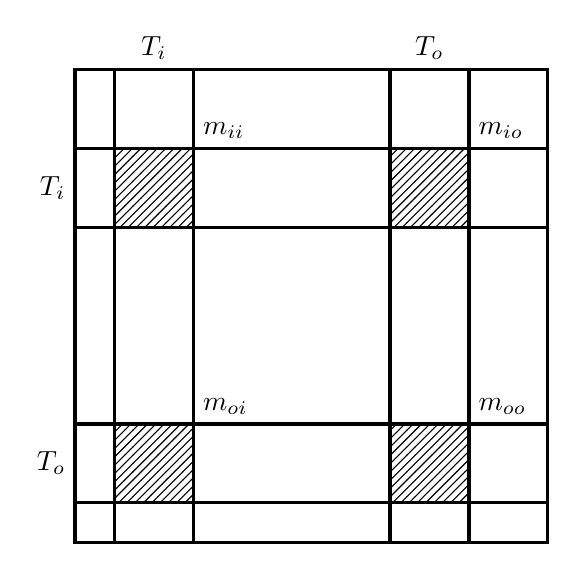
\begin{tikzpicture}[scale=1.0]
\draw[draw=none,pattern=north east lines] (0.5,0.5)  rectangle (1.5,1.5);
\draw[draw=none,pattern=north east lines] (4,0.5)  rectangle (5,1.5);
\draw[draw=none,pattern=north east lines] (0.5,4)  rectangle (1.5,5);
\draw[draw=none,pattern=north east lines] (4,4)  rectangle (5,5);
\draw[very thick] (0,0)  rectangle (6,6);
\draw[very thick] (0,0.5) -- (6,0.5);
\draw[very thick] (0,1.5) -- (6,1.5);
\draw[very thick] (0,4) -- (6,4);
\draw[very thick] (0,5) -- (6,5);
\draw[very thick] (0.5,0) -- (0.5,6);
\draw[very thick] (1.5,0) -- (1.5,6);
\draw[very thick] (4,0) -- (4,6);
\draw[very thick] (5,0) -- (5,6);
\node[left] at (0,4.5) {$T_{i}$};
\node[left] at (0,1) {$T_{o}$};
\node[above] at (1,6) {$T_{i}$};
\node[above] at (4.5,6) {$T_{o}$};
\node[above right] at (1.5,5) {$m_{ii}$};
\node[above right] at (5,5) {$m_{io}$};
\node[above right] at (1.5,1.5) {$m_{oi}$};
\node[above right] at (5,1.5) {$m_{oo}$};
\end{tikzpicture}\hspace{0.1\textwidth}
\end{center}
\caption{Matrix block contributions computed by \lstinline{jacobian_skeleton}.}
\label{fig:MatrixBlocks}
\end{figure}

The method has the following interface:
\lstinputlisting[linerange={189-195},
basicstyle=\ttfamily\small,
frame=single,
backgroundcolor=\color{listingbg}]{../src/nonlinearpoissonfv.hh}
It is very similar to \lstinline{alpha_skeleton} except that four containers
are passed where the matrix entries of the four blocks need to be stored.

The computation of distance of cell centers and the face volume are
exactly the same as in \lstinline{alpha_skeleton}.
Then the matrix entries are given by:
\lstinputlisting[linerange={217-221},
basicstyle=\ttfamily\small,
frame=single,
backgroundcolor=\color{listingbg}]{../src/nonlinearpoissonfv.hh}

\subsubsection*{Method \lstinline{jacobian_apply_skeleton}}

The \lstinline{jacobian_apply_skeleton} method needs to
compute the local Jacobian contributions and multiply them with
a given coefficient vector. It has the following interface
\lstinputlisting[linerange={225-231},
basicstyle=\ttfamily\small,
frame=single,
backgroundcolor=\color{listingbg}]{../src/nonlinearpoissonfv.hh}
\lstinline{x_i}, \lstinline{x_o} are the linearization point
and \lstinline{z_i}, \lstinline{z_o} are the coefficients to multiply with.

As the skeleton terms are linear with respect to degrees of freedom
the Jacobian does not depend on the linearization point and
we may reuse the \lstinline{alpha_skeleton} method here:
\lstinputlisting[linerange={234-234},
basicstyle=\ttfamily\small,
frame=single,
backgroundcolor=\color{listingbg}]{../src/nonlinearpoissonfv.hh}

\subsubsection*{Method \lstinline{alpha_boundary}}

The \lstinline{alpha_boundary} method is also new. It corresponds
to the fourth sum on the right hand side of equation \eqref{eq:res_form_final}
which is again linear in the degrees of freedom.
The interface is now:
\lstinputlisting[linerange={239-243},
basicstyle=\ttfamily\small,
frame=single,
backgroundcolor=\color{listingbg}]{../src/nonlinearpoissonfv.hh}
The residual contribution depends only on quantities on the inside
element of the intersection.

First we need to check whether the face is on the Dirichlet boundary:
\lstinputlisting[linerange={246-250},
basicstyle=\ttfamily\small,
frame=single,
backgroundcolor=\color{listingbg}]{../src/nonlinearpoissonfv.hh}

Then the distance from face center to cell center is computed:
\lstinputlisting[linerange={252-260},
basicstyle=\ttfamily\small,
frame=single,
backgroundcolor=\color{listingbg}]{../src/nonlinearpoissonfv.hh}
and the residual contribution can be accumulated:
\lstinputlisting[linerange={262-266},
basicstyle=\ttfamily\small,
frame=single,
backgroundcolor=\color{listingbg}]{../src/nonlinearpoissonfv.hh}

\subsubsection*{Method \lstinline{jacobian_boundary}}

The \lstinline{jacobian_boundary} method computes
the Jacobian contributions resulting from boundary face integrals
and has the following interface:
\lstinputlisting[linerange={270-274},
basicstyle=\ttfamily\small,
frame=single,
backgroundcolor=\color{listingbg}]{../src/nonlinearpoissonfv.hh}
The interface is the same as for \lstinline{alpha_boundary} except that
a matrix container is passed as the last argument.

As the contributions only depend on test and trial functions
of the inside element there is only contribution to one
matrix entry:
\lstinputlisting[linerange={298-298},
basicstyle=\ttfamily\small,
frame=single,
backgroundcolor=\color{listingbg}]{../src/nonlinearpoissonfv.hh}

\subsubsection*{Method \lstinline{jacobian_apply_boundary}}

Finally, the \lstinline{jacobian_apply_boundary} does a
matrix-free Jacobian times vector multiplication. Due to linearity
we can reuse the \lstinline{alpha_boundary} method:
\lstinputlisting[linerange={302-311},
basicstyle=\ttfamily\small,
frame=single,
backgroundcolor=\color{listingbg}]{../src/nonlinearpoissonfv.hh}

\subsection{Running the Example}

Figure \ref{fig:Bunt} shows results for three different values of $\eta$ on a relatively
coarse mesh. Clearly, the piecewise constant approximation can be seen.

\begin{figure}[h]
\begin{center}
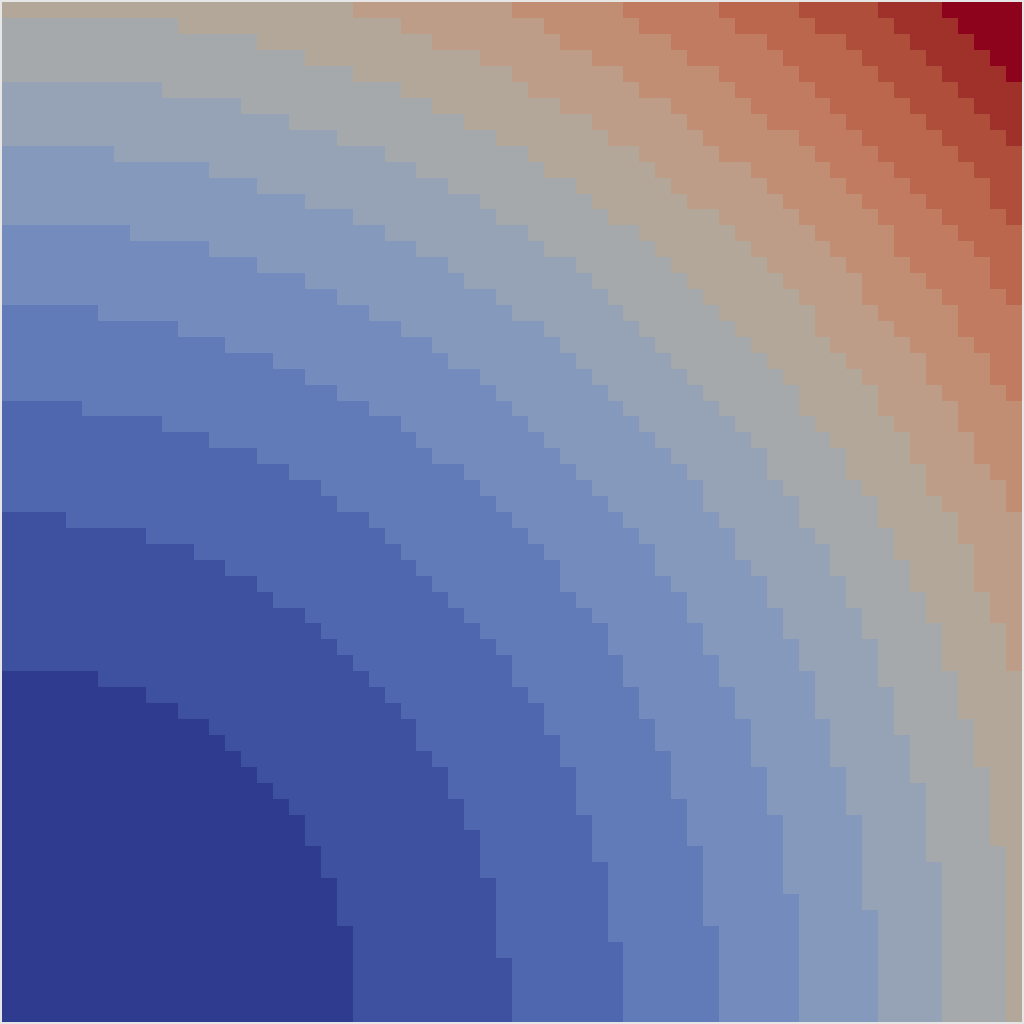
\includegraphics[width=0.32\textwidth]{eta0}\hfill
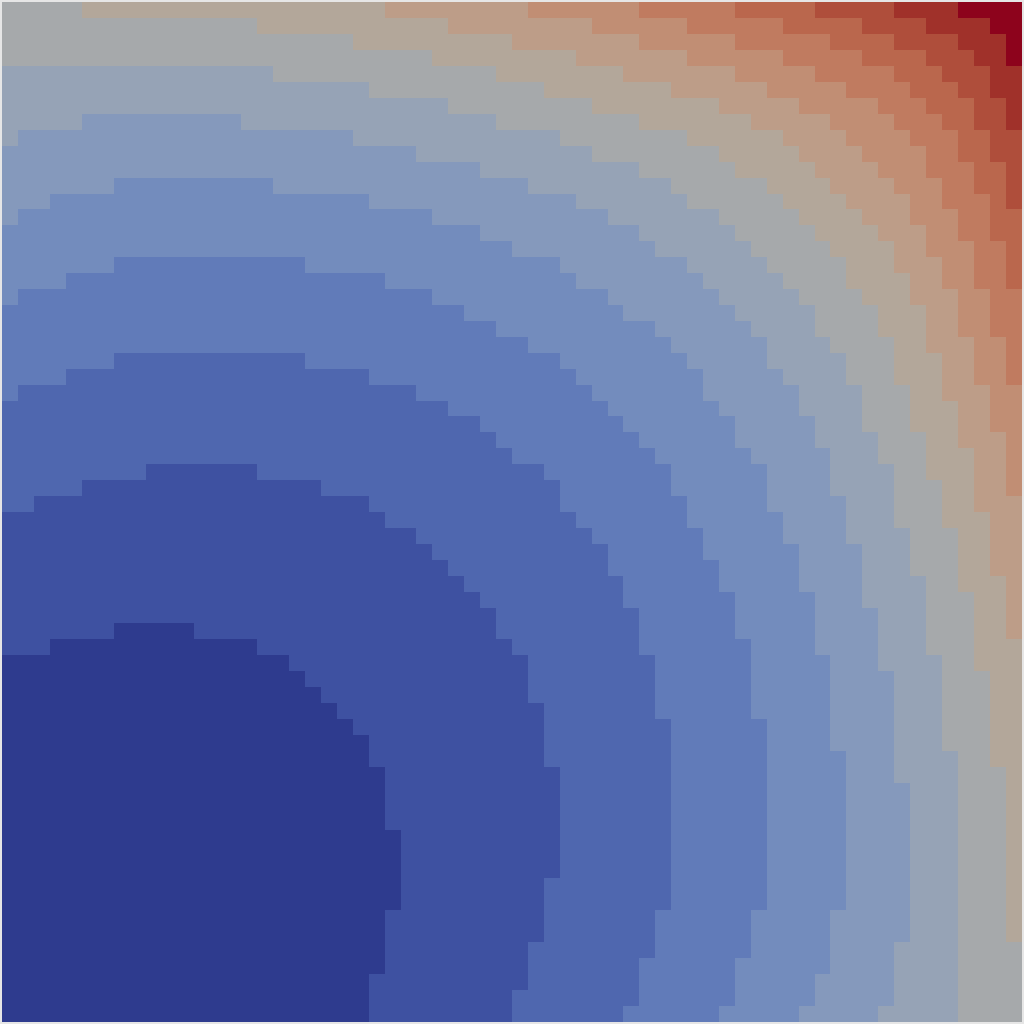
\includegraphics[width=0.32\textwidth]{eta10}\hfill
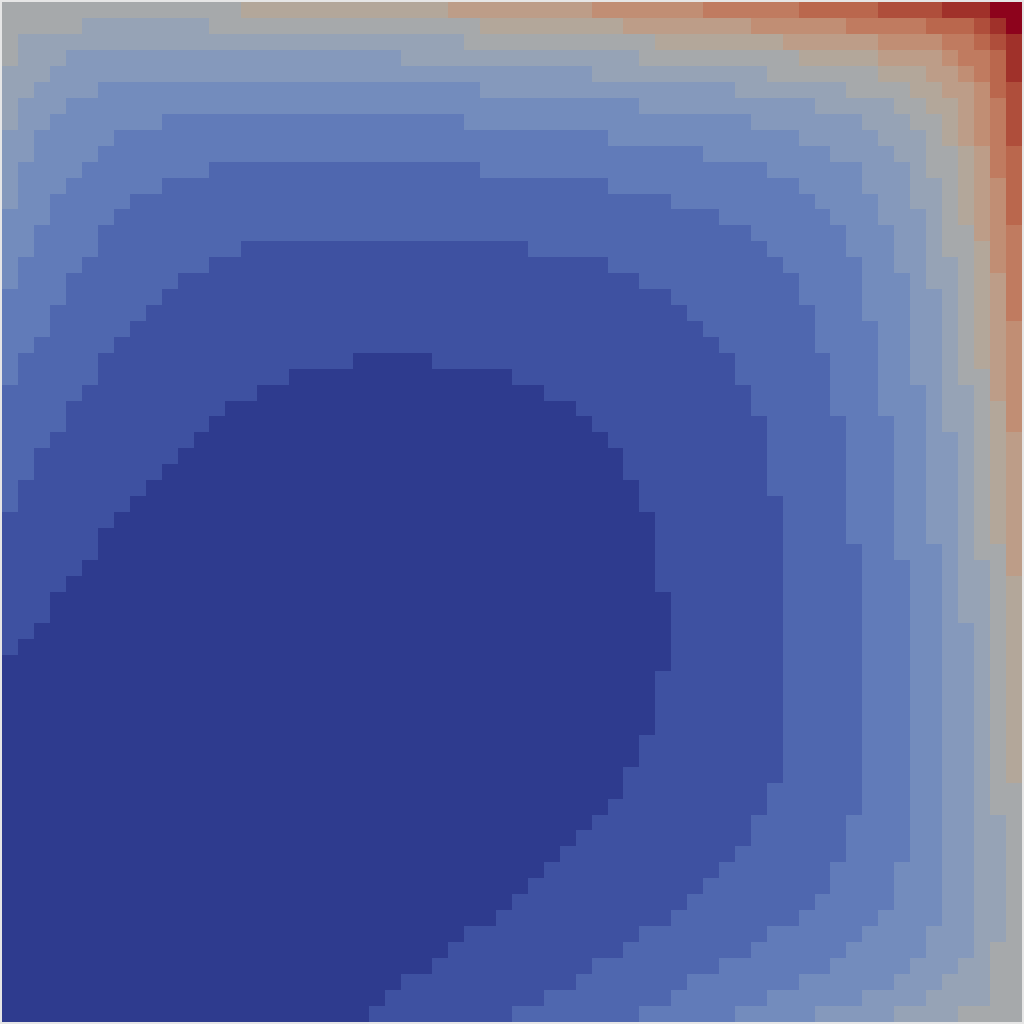
\includegraphics[width=0.32\textwidth]{eta100}
\end{center}
\caption{Illustration of the influence of the parameter $\eta$
in nonlinearity on the solution. $\eta=0$ (left), $\eta=10$ (middle), $\eta=100$ (right).}
\label{fig:Bunt}
\end{figure}

\begin{figure}
\caption{Comparison of conforming finite element and cell-centered finite volume
method}
\label{fig:Compare}
\begin{center}
\begin{tabular}{l|r|r}
 & \multicolumn{1}{r|}{$Q1$ conforming FEM} & \multicolumn{1}{r}{cell-centered FV} \\
 \hline
 \# DOF & 263169 & 262144 \\
 Matrix assembly time & 0.87 & 0.20 \\
 Time per iteration & 0.10 & 0.08 \\
 \# Linear Iterations & 15 & 9 \\
 \# Newton Iterations & 5 & 5 \\
 Total time & 16.83 & 6.95
\end{tabular}
\end{center}
\end{figure}

The table in Figure \ref{fig:Compare} shows a run-time comparison
of the $Q_1$ conforming finite element method with numerical Jacobian
from tutorial 01 with the cell-centered finite volume method implemented here
on a $512^2$ mesh in $2d$ and $\eta=100$:
One can see that matrix assembly is five times faster, both due to less work
per element and analytic Jacobian. The time per iteration in the algebraic multigrid
solver is about the same but the number of iterations is less for the FV scheme.
In total the FV scheme is more than two times faster.

\section{Outlook}

Here are some suggestions how to test and modify this example:
\begin{itemize}
\item Compare the convergence of Newton's method in tutorial 01 and 02. Does the
exact Jacobian in combination with a different discretization scheme make any difference?
\item Implement a convection term with upwinding. The equation in strong conservative
form is
$$ \nabla\{ \vec\beta u - \nabla u\} + q(u) = f $$
where $\vec\beta(x)$ is a given (divergence free) velocity field.

In the residual form the full upwind discretization is realized by the following
term:
$$r_h^{conv}(u,v) = \sum_{F\in\mathcal{F}_h^i} \vec\beta(x_F) u^\uparrow_F
\bigl[v(x_{T_F^-}) - v(x_{T_F^+})\bigr] |F|$$
where the upwind value is
$$ u^\uparrow_F = \left\{\begin{array}{ll}
u(x_F^-) & \vec\beta(x_F)\cdot\nu_F\geq 0 \\
u(x_F^+) & \text{else}
\end{array}\right . .$$
\end{itemize}

% bibtex bibliography
%\bibliographystyle{plain}
%\bibliography{tutorial02.bib}

\end{document}
